\begin{frame}[fragile]
  \frametitle{Colecciones}

  \begin{enumerate}[2.]
    \item Tuplas    
  \end{enumerate}


  Una tupla es una lista inmutable, es decir, no puede modificarse de ning\'un modo despu\'es de su creaci\'on. Se define igual que una lista, salvo que el conjunto se encierra entre par\'entesis en lugar de entre corchetes. Tambi\'en tienen un orden definido.

  \begin{itemize}
    \item Ejemplo:
  \end{itemize}

  \begin{figure}
    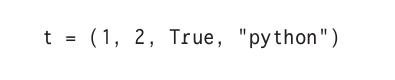
\includegraphics[width=0.6\textwidth]{Imagenes/Tuplas.jpg}
    \caption{\label{fig:Ejemplo2}Creaci\'on de una tupla en Python.}
  \end{figure}  
 
 
\end{frame}
